\chapter{Setting up and Maintaining Digifiz Replica} \label{ch:replica-setup}

Classic Digifiz Replica dashboards require regular care to remain reliable.

\section{Front Panel Care}

The plexiglass screen is UV printed and can be marred by sharp objects.
Avoid abrasive cleaners and protect the panel during installation or storage; cosmetic damage is not covered by warranty.

\section{Backup Battery}

The integrated DS3231 real-time-clock module uses a replaceable CR2032 cell with an expected life of approximately four years.
When the dashboard begins losing time after each power cycle, remove the rear cover, replace the battery without disconnecting the harness, and dispose of the depleted cell responsibly.

\section{USBasp Programming}

Each dashboard ships with a USBasp programmer and a pre-installed wiring harness.
Install the required driver (for example via \url{https://myrobot.ru/downloads/driver-usbasp-v-2.0-usb-isp-windows-7-8-10-xp.php}) before connecting the programmer to a Windows host.
Connecting the programmer powers the dashboard, allowing firmware updates and diagnostic checks without the vehicle.

\begin{figure}[htbp]
    \centering
    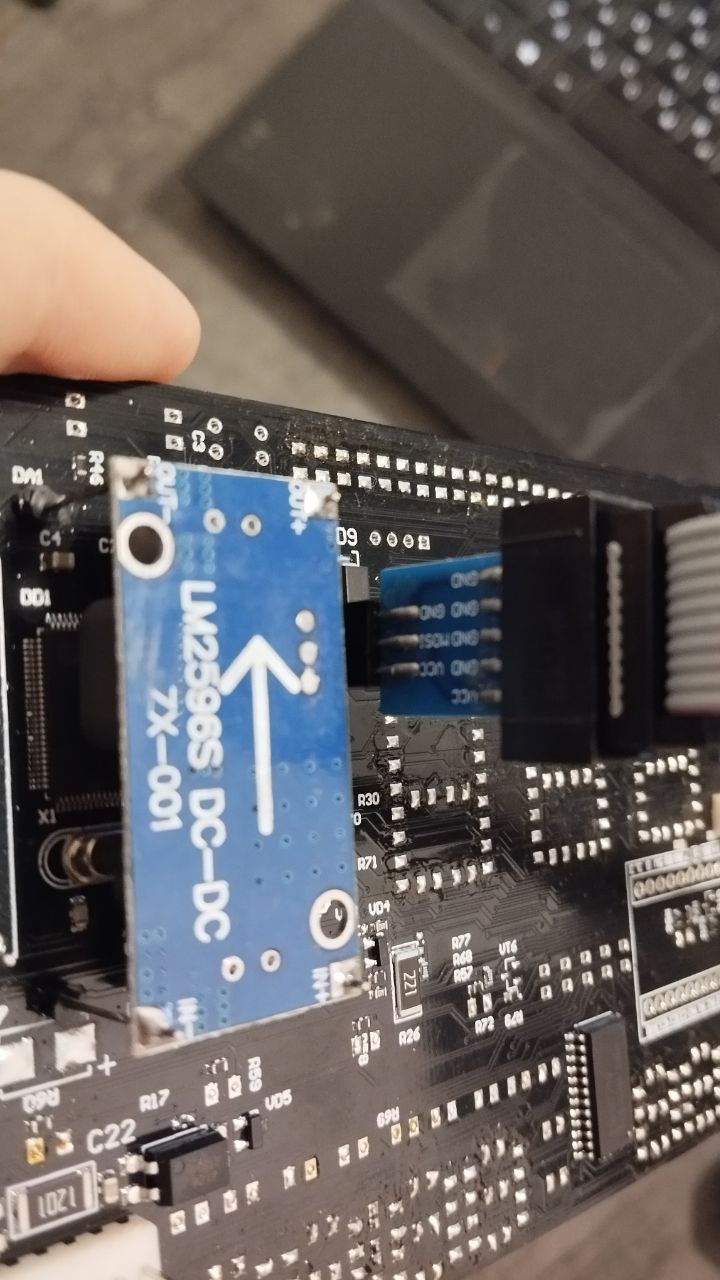
\includegraphics[width=0.35\textwidth]{digifiz_manual/image048.png}
    \caption{USBasp programming cable orientation on the classic Replica PCB.}
    \label{fig:usbasp-orientation}
\end{figure}

The recommended \texttt{avrdude} invocation for reflashing an ATmega~2560-based dashboard (wrapped across two lines for readability) is:
\begin{verbatim}
avrdude -c usbasp -p m2560 -e -U lfuse:w:0xff:m -U hfuse:w:0x99:m
    -U efuse:w:0xff:m -U flash:w:Digifiz.ino.mega.hex
\end{verbatim}

After a successful flash, press the capacitive touch button four or five times to initialise the MFA memory blocks.
If the memory fails to populate, repeat the flashing procedure or issue the Bluetooth command \verb|252 0| to perform a factory reset.

\section{Firmware Availability}

Compiled firmware images and source code are maintained at \url{https://github.com/Sgw32/DigifizReplica} (\Cref{ch:description}).
Keep a record of the odometer value and restore it with command \verb|11 <mileage>| after reflashing when necessary.

\chapter{Typical Situations for Setting up the Digifiz Panel Replica (without Next)} \label{ch:replica-scenarios}

The scenarios below summarise frequent support questions for classic Replica dashboards.

\begin{description}
    \item[Bluetooth module not visible] Confirm that the host uses Bluetooth Classic rather than BLE.
          iOS devices cannot connect to the Bluetooth~2.0 module.
    \item[Commands rejected] Firmware builds from 2024 and newer require unlocking with \verb|234 123| before accepting configuration commands.
    \item[Speed or RPM calibration] Adjust \texttt{PARAMETER\_SPEEDCOEFFICIENT} with \verb|1 <gps_value>| and \texttt{PARAMETER\_RPMCOEFFICIENT} with \verb|0 <value>| or \verb|22 <value>|, using the same approach as Replica Next.
    \item[Manual brightness adjustment] Disable automatic brightness with \verb|13 0| and set \verb|14 15| for maximum brightness.
          Re-enable automatic control with \verb|13 1| if required.
    \item[Clock adjustment] Enter \verb|255 <hours>| followed by \verb|254 <minutes>| through Serial Bluetooth Terminal.
    \item[Fuel gauge issues] With the battery disconnected, verify the sender resistance on the harness (30--300~\ohm{}) and inspect for shorts.
          Check the signal path to the main board and clean contacts if needed.
    \item[Fuel flow accuracy] The optional flow sensor relies on intake manifold pressure data and otherwise produces approximate readings.
    \item[Coolant temperature calibration] Tune \texttt{PARAMETER\_COOLANT\_MIN\_R} and \texttt{PARAMETER\_COOLANT\_MAX\_R} experimentally to suit the vehicle (for example, \verb|27 30|).
\end{description}

For additional parameter defaults and configuration details, refer to \Cref{tbl:next-commands,tbl:next-defaults} and the classic Replica command list in \Cref{appendix:reference}.
